\section{Resultados}
% Figuras y tablas generadas por codigo/notebooks/03_frente_C_clasificacion.ipynb
% y 04_frente_C_hipotesis.ipynb. Se guardan solas en figuras/.

\subsection{Preprocesamiento y descriptores}
\textbf{Línea eléctrica y filtrado.} El pico en \SI{50}{\hertz} superó los \SI{3}{\decibel} en el 95\,\% de los pares paciente y canal (mediana \SI{17,5}{\decibel}), mientras que en \SI{60}{\hertz} la mediana fue de \SI{0,1}{\decibel} (Fig.~\ref{fig:linea}), por lo que el notch se fijó en \SI{50}{\hertz}. Con un pasa-altos de \SI{0,5}{\hertz}, una onda de \SI{-80}{\micro\volt} se reducía a \SI{-57}{\micro\volt} y quedaba debajo del umbral de detección, mientras que con \SI{0,2}{\hertz} conservó \SI{-72}{\micro\volt}. Los registros que el equipo filtró con un pasa-bajos de \SI{35}{\hertz} y los que filtró con uno de \SI{128}{\hertz} difirieron en \SI{0,3}{\decibel} a \SI{30}{\hertz}, donde terminan las bandas de los descriptores, por lo que se trataron todos igual.

\textbf{Saturación.} En el paciente mediano solo el 0,05\,\% de las muestras de EEG llegó al borde del rango, pero eso alcanzó para afectar al 2,6\,\% de las épocas, tomando el canal más afectado de cada paciente. El peor caso fue SN020, con el 37\,\% de las épocas. No se descartaron épocas, porque hay que clasificarlas todas, pero los tramos de más de \SI{500}{\micro\volt} quedaron fuera del ajuste del filtro ocular y de la plantilla cardíaca.

\begin{figure}[htbp]
  \centering
  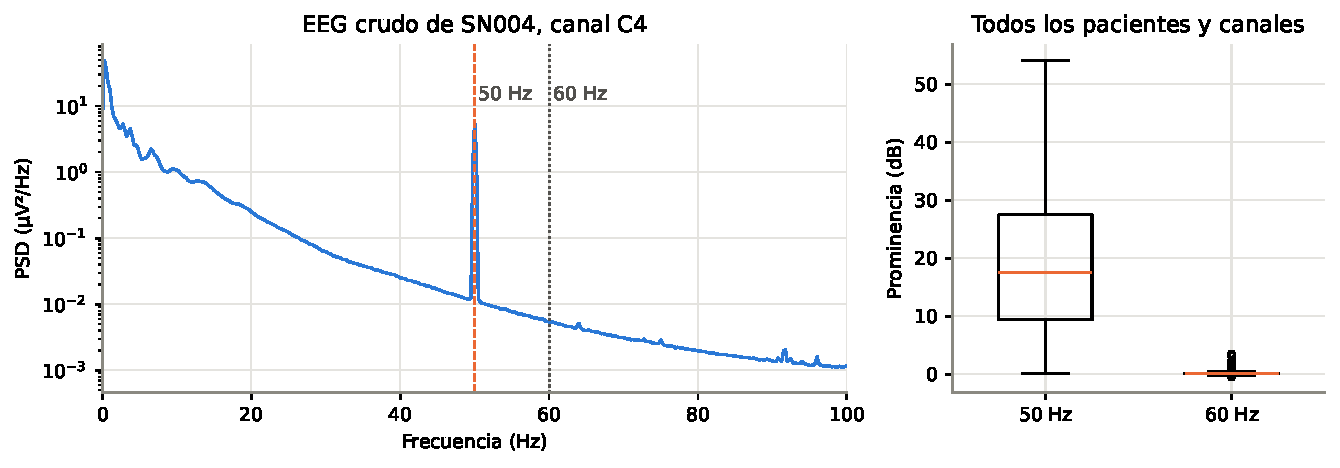
\includegraphics[width=0.9\textwidth]{a_linea_electrica}
  \caption{Espectro crudo de un paciente (izquierda) y prominencia de 50 y \SI{60}{\hertz} en los pacientes de entrenamiento (derecha).}
  \label{fig:linea}
\end{figure}

\textbf{Artefacto ocular.} Corregir toda la noche redujo un 6,5\,\% (Wiener) y un 14\,\% (NLMS) las ondas lentas detectadas en N3. Wiener con compuerta conservó N3 (de 5018 a 4994 ondas, en 12 pacientes) y redujo un 19\,\% las detecciones en REM, que eran movimientos oculares (Fig.~\ref{fig:ondas}). NLMS con compuerta aumentó la potencia delta en W y N1, por lo que se adoptó Wiener.

\begin{figure}[htbp]
  \centering
  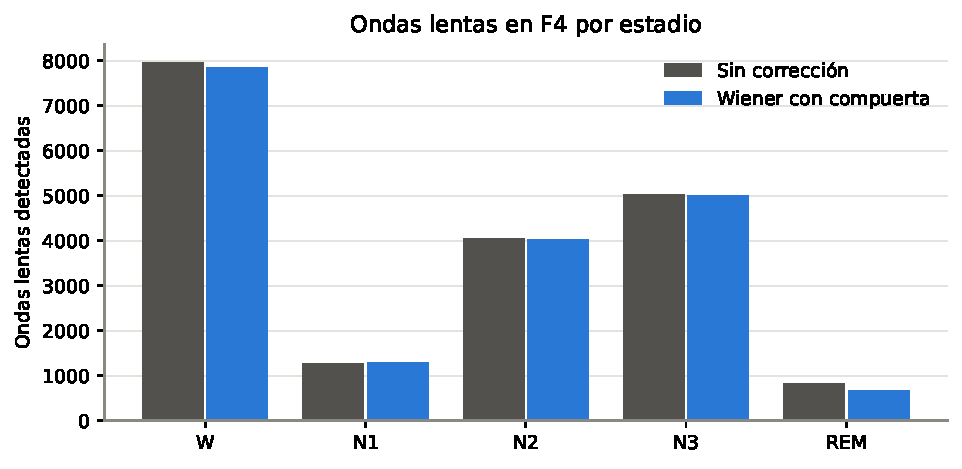
\includegraphics[width=0.6\textwidth]{a_ondas_por_estadio}
  \caption{Ondas lentas detectadas en F4 por estadio, antes y después de la corrección ocular.}
  \label{fig:ondas}
\end{figure}

\textbf{Artefacto cardíaco.} El promedio sincronizado mostró el QRS y la onda T en los 12 pacientes analizados (Fig.~\ref{fig:cardiaco}). En F4 su amplitud mediana fue de \SI{17}{\micro\volt} pico a pico, unas 40 veces la del control con instantes al azar (\SI{0,4}{\micro\volt}), lo que responde a la duda planteada en la devolución. C3, referido a M2, tuvo la mitad de artefacto que los canales referidos a M1. La remoción lo redujo a \SI{1,6}{\micro\volt} (91\,\%) sin cambiar la potencia delta, y quitó más potencia en REM que en W, con \SI{0,55}{\decibel} contra \SI{0,06}{\decibel} en alfa de O2 y \SI{0,62}{\decibel} contra \SI{0,16}{\decibel} en sigma de C4.

\begin{figure}[htbp]
  \centering
  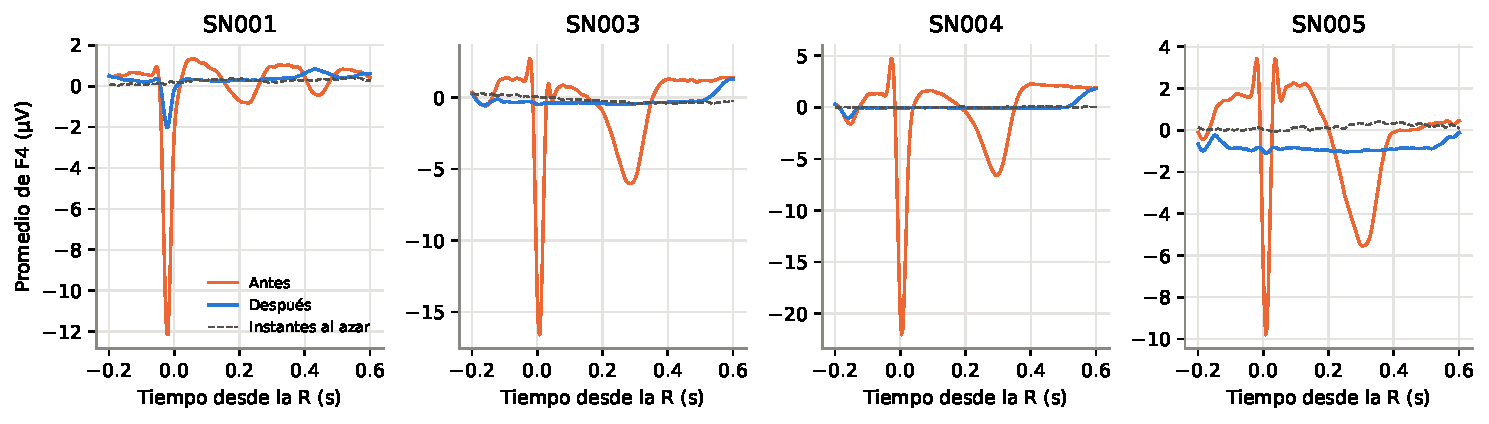
\includegraphics[width=\textwidth]{a_promedio_latidos}
  \caption{Promedio de F4 alrededor de cada latido antes y después de la remoción, y en instantes al azar como control.}
  \label{fig:cardiaco}
\end{figure}

\textbf{Segmentación.} La marca de no estacionariedad abarcó el 10\,\% de las épocas de entrenamiento, con 25\,\% en W y 3\,\% en N3, y fue más frecuente en las épocas de transición entre estadios (17,5\,\% contra 7,5\,\%). En las épocas marcadas el clasificador acertó el 28\,\% contra el 45\,\% de las no marcadas. Un tercio de las épocas marcadas de W, N1, N2 y REM se clasificó como N3, porque la regla de N3 tomó las deflexiones grandes como ondas lentas.

\textbf{Latidos y HRV.} En los 12 pacientes analizados, Pan-Tompkins detectó entre 24\,700 y 37\,900 latidos por noche, con RR medianos entre 0,69 y \SI{1,06}{\second}. El descarte por forma sacó una mediana del 4,9\,\% de los latidos, y después de filtrar los intervalos se conservó al menos el 90\,\% en 10 de los 12 pacientes. La excepción fue SN001, con el 47\,\%, porque tiene un ritmo muy irregular. El 24\,\% de sus intervalos es más de un 20\,\% más corto que el de sus vecinos, contra una mediana del 1,8\,\% en los demás. El cociente LF/HF fue menor en N3 y mayor en REM, como se esperaba, con percentiles medianos de 25 y 70 dentro de la noche. HF bajó en REM pero no subió en N3, por lo que la regla de REM usa el cociente.

\textbf{Descriptores por estadio.} Para ver si cada descriptor separa los estadios en todos los pacientes y no solo en uno, se estandarizó cada descriptor dentro de cada noche y se promedió por estadio en cada uno de los 56 pacientes de entrenamiento, entre luces apagadas y encendidas (Fig.~\ref{fig:huella}). El descriptor más consistente fue la pendiente del espectro, que en C4 pasó de una mediana de $-1{,}36$ en W a $-2{,}66$ en N3 y fue más empinada en N3 que en W en los 56 pacientes. La potencia $\delta$ relativa en F4 fue máxima en N3 en 49 pacientes y la amplitud del EMG fue mínima en REM en 43. La $\alpha$ relativa en O2 fue máxima en W solo en 31, y la energía del EOG resultó más alta en W que en REM ($+0{,}92$ contra $+0{,}46$ desvíos), de modo que ninguno de los dos alcanza por sí solo para reconocer esos estadios.

\begin{figure}[htbp]
  \centering
  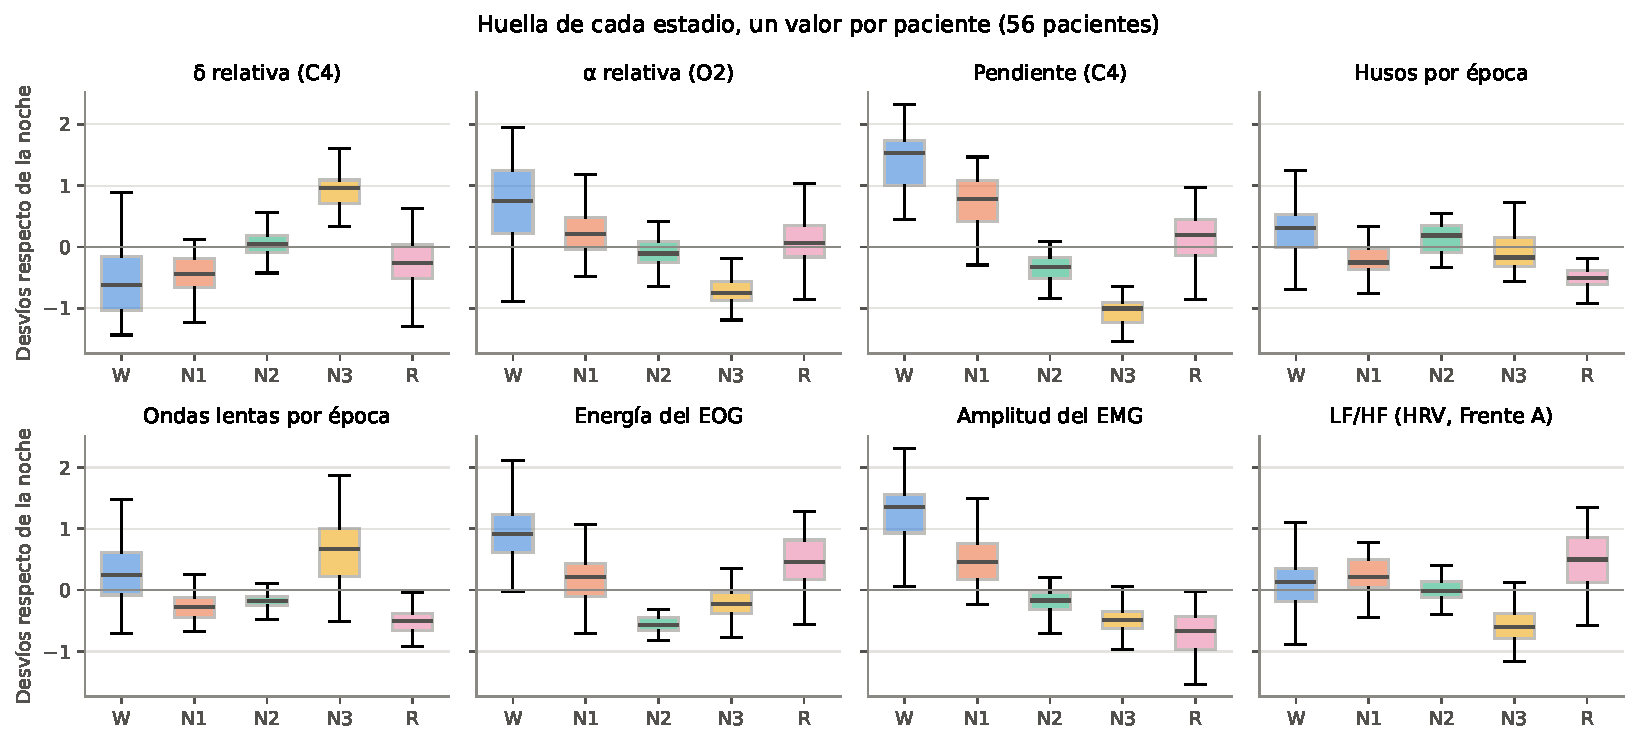
\includegraphics[width=\textwidth]{b_huella_pacientes}
  \caption{Descriptores estandarizados dentro de cada noche, un valor por paciente y por estadio (56 pacientes de entrenamiento). La línea horizontal marca el valor medio de la noche.}
  \label{fig:huella}
\end{figure}

\textbf{Husos y ondas lentas en vigilia.} Los dos detectores encontraron eventos en W. La mediana entre pacientes fue de 1,10 husos por época en W y de 0,99 en N2, y W superó a N2 en 34 de los 56 pacientes. Las ondas lentas fueron 2,42 por época en N3 y 1,79 en W, y N3 superó a todos los demás estadios solo en 33 pacientes. Dentro de W, las épocas con dos o más husos tuvieron un EMG más alto que las que no tenían ninguno en los 56 pacientes (mediana de 17 contra \SI{7}{\micro\volt}) y menos $\alpha$ en O2 en 55 (0,04 contra 0,15). Con las ondas lentas el resultado fue el mismo. En el paciente de ejemplo, además, las detecciones de W tuvieron la misma frecuencia que las de N2, cerca de \SI{13}{\hertz}, y la corrección ocular redujo un 75\,\% las ondas lentas de REM pero solo un 7\,\% las de W. Las detecciones de vigilia corresponden entonces a vigilia activa, con movimiento y tensión muscular, y no al ritmo $\alpha$ ni a movimientos oculares.

\textbf{Woody sobre ondas reales.} En los 55 pacientes de entrenamiento con al menos cinco ondas lentas en N3, la plantilla de Woody tuvo un valle menos profundo que el promedio ordinario (mediana de $-78{,}9$ contra \SI{-83,1}{\micro\volt}), porque cada onda se recorta centrada en su mínimo y el promedio ordinario suma ahí el ruido de todas. El algoritmo convergió antes de las 20 iteraciones en 25 pacientes. En los demás siguió moviendo unas pocas ondas muy deformadas, que saltan entre posiciones sin estabilizarse, y en el paciente mediano el 0,4\,\% de las ondas quedó en el corrimiento máximo de \SI{0,25}{\second}. Entre las épocas con ondas, la similitud con la plantilla fue parecida en todos los estadios (mediana entre 0,74 y 0,79).

\subsection{Clasificación}
\pendiente{Comentar la distribución de estadios (\texttt{c\_distribucion\_estadios}) y los umbrales elegidos (\texttt{c\_eleccion\_umbrales}).}

% \begin{figure}[htbp]
%   \centering
%   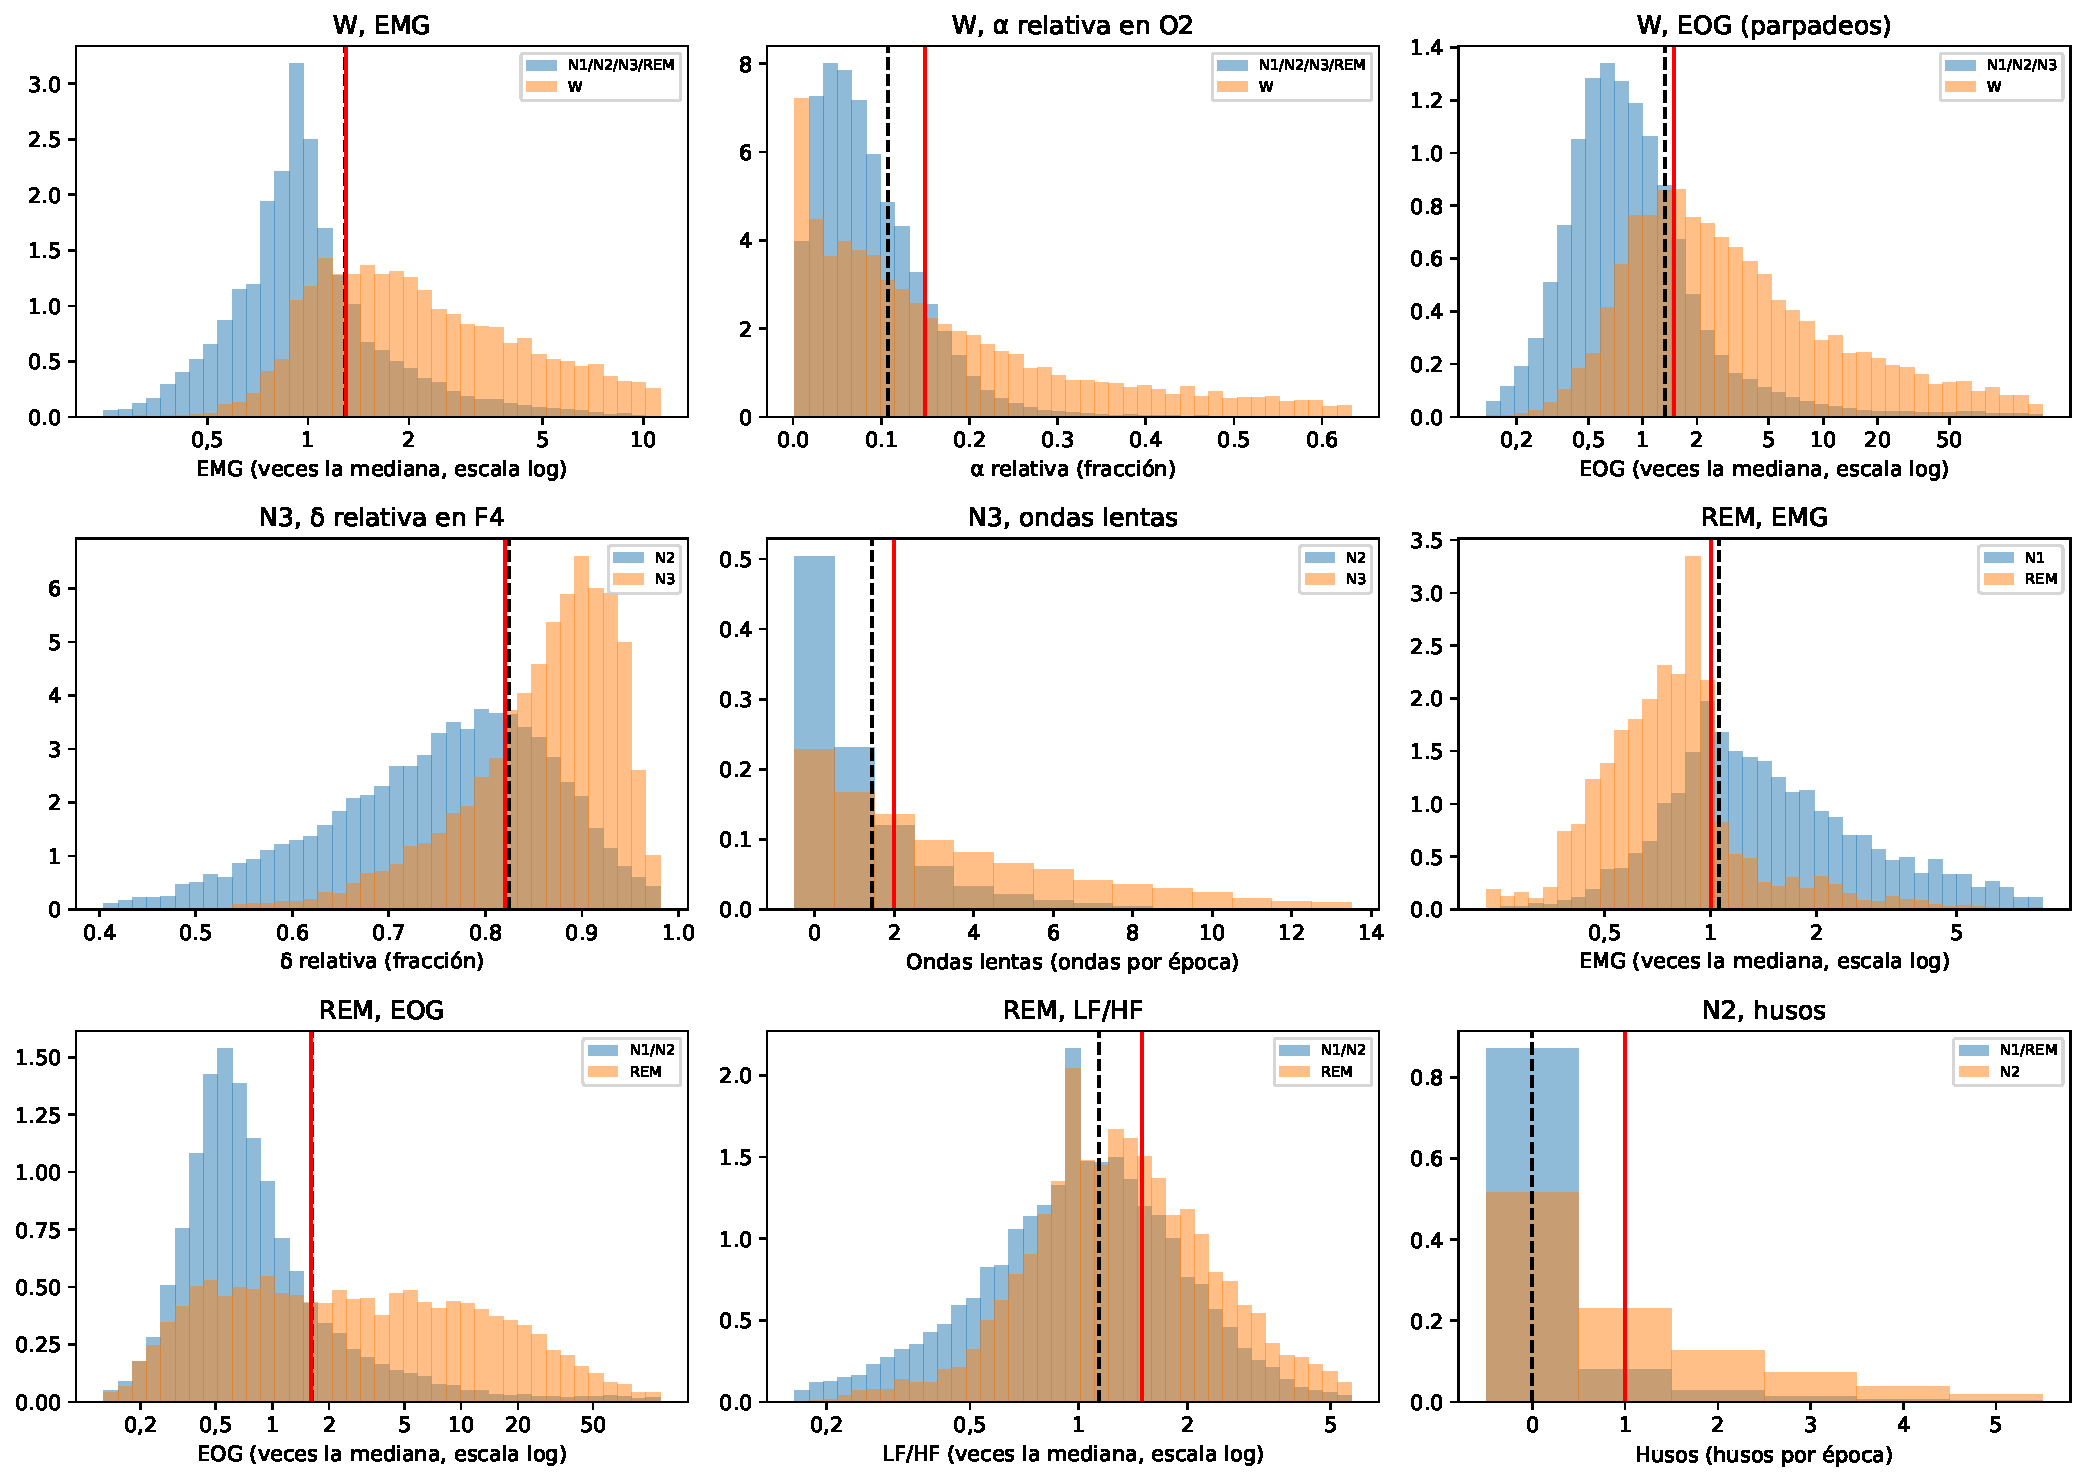
\includegraphics[width=\textwidth]{c_eleccion_umbrales}
%   \caption{Histogramas de cada descriptor en los estadios que separa cada regla (pacientes de entrenamiento). Punteada: cruce de los histogramas; roja: umbral elegido.}
%   \label{fig:umbrales}
% \end{figure}

\begin{table}[htbp]
  \centering
  \caption{Acuerdo con los técnicos sobre los \pendiente{14} pacientes de prueba.}
  \label{tab:resultados}
  \begin{tabular}{lcccccc}
    \toprule
    & $\kappa$ & F1 W & F1 N1 & F1 N2 & F1 N3 & F1 REM \\
    \midrule
    Reglas                  & -- & -- & -- & -- & -- & -- \\
    Reglas + moda           & -- & -- & -- & -- & -- & -- \\
    Reglas + continuidad    & -- & -- & -- & -- & -- & -- \\
    \midrule
    Técnicos HMC~\cite{alvarez2021}        & 0,74 & & & & & \\
    Red de referencia~\cite{alvarez2021}   & 0,79 & & & & & \\
    \bottomrule
  \end{tabular}
\end{table}

% \begin{figure}[htbp]
%   \centering
%   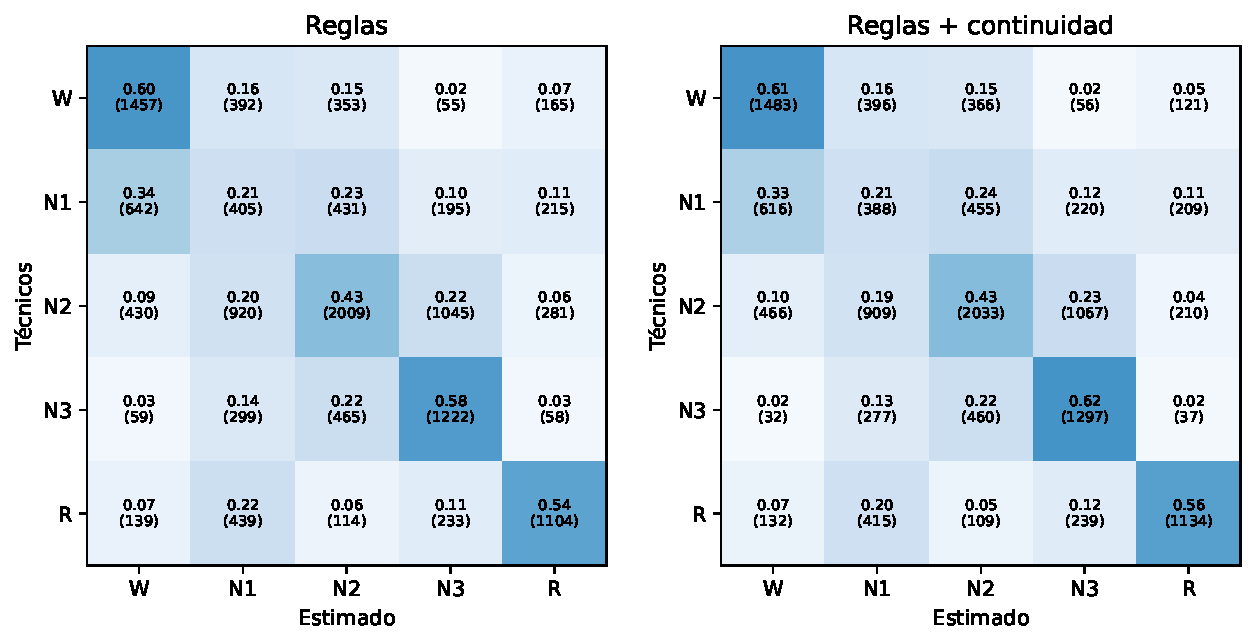
\includegraphics[width=\textwidth]{c_matrices_confusion}
%   \caption{Matrices de confusión normalizadas por fila (estadio de los técnicos).}
%   \label{fig:confusion}
% \end{figure}

% \begin{figure}[htbp]
%   \centering
%   \includegraphics[width=\textwidth]{c_hipnograma_SNxxx}
%   \caption{Hipnograma de un paciente de prueba: técnicos, reglas y reglas con suavizado.}
%   \label{fig:hipnograma}
% \end{figure}

% \begin{figure}[htbp]
%   \centering
%   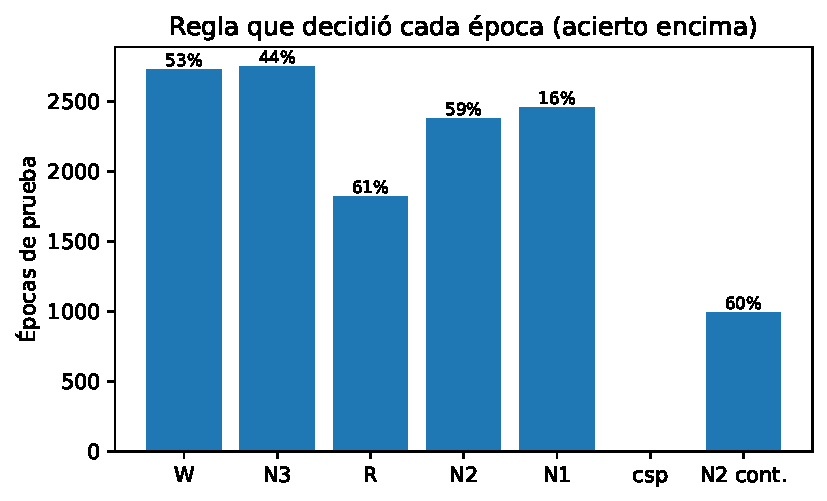
\includegraphics[width=0.7\textwidth]{c_uso_reglas}
%   \caption{Cantidad de épocas de prueba que decidió cada regla y fracción de aciertos.}
%   \label{fig:uso_reglas}
% \end{figure}

\subsection{Verificación de hipótesis}

\begin{table}[htbp]
  \centering
  \caption{Comparaciones paciente por paciente (Wilcoxon).}
  \label{tab:hipotesis}
  \begin{tabular}{llccc}
    \toprule
    & Medida & Variante A & Variante B & $p$ \\
    \midrule
    H1 & Variación por banda     & Multitaper: 0,142 & Welch: 0,148      & 0,0001 \\
       & Variación por frecuencia & Multitaper: 0,182 & Welch: 0,220     & 0,0001 \\
    H2 & Error de forma          & Woody: 0,28      & Promedio: 0,42   & 0,049 \\
    H3 & F1 de N1                & Con desempate: 0,21 & Sin desempate: 0,20 & 0,13 \\
       & F1 de REM               & Con desempate: 0,54 & Sin desempate: 0,58 & 0,033 \\
    H4 & Residuo cardíaco (\si{\micro\volt}) & Después: -- & Antes: -- & -- \\
       & $\kappa$                & Con etapas: -- & Sin etapas: -- & -- \\
    \bottomrule
  \end{tabular}
\end{table}
